% !TEX root = ../main.tex
\subsection{Cuts}
\label{13.20::cuts}
    In order to enhance the relevance of particles for the analysis presented in this work, three types of cuts are applied:
    \begin{itemize}
        \item
            General cuts:
            These cuts are designed to exclude poorly reconstructed particles.
        \item
            Geometry cuts:
            These cuts define the region from which the reconstruction data is considered valid and useful for the analysis.
        \item
            DIS cuts:
            These cuts narrow down the analysis region to focus specifically on DIS.
    \end{itemize}
    By applying these cuts, the analysis can be focused on particles that meet the criteria for good reconstruction, fall within the desired geometry range, and are relevant to the DIS process.

    % !TEX root = ../main.tex
\subsubsection{General Cuts}
\label{13.21::general_cuts}
    For this analysis, only two cuts are considered as ``general''.
    The first cut involves filtering out particles with PID values of 0 or 45.
    In CLAS12 reconstruction, these specific PID values are assigned to particles whose identification could not be successfully determined.

    The second cut aims to exclude particles with imprecise tracking and is defined as follows
    \begin{equation*}
        \frac{\chi^2}{\text{NDF}} < 15,
    \end{equation*}
    where $\chi^2$ represents the final result from the $\chi^2$-test used in the Kalman filter fit of the tracking algorithm, as described in Section \ref{11.230::offline_reconstruction}.
    The term NDF denotes the number of degrees of freedom associated with this same fit.

    By applying these two cuts, particles with undetermined or uncertain identification (PID values of 0 or 45) and those with poor tracking precision (exceeding the specified $\chi^2$/NDF threshold) are excluded from the analysis.

    % !TEX root = ../main.tex
\subsubsection{Geometry Cuts}
\label{13.22::geometry_cuts}
    Three geometry cuts are derived to constrain the reconstructed particle's vertex position.
    The first two cuts ensure that the vertex is located along the beamline, while the third cut restricts it to the acceptance region of the FMT.

    The first cut guarantees that the vertex is close to the beamline and is defined as:
    \begin{equation*}
        \sqrt{v_x^2 + v_y^2} < 4 \text{ cm},
    \end{equation*}
    where $v_x$ and $v_y$ represent the $x$ and $y$ coordinates of the vertex position, respectively.

    The second cut ensures that the vertex originates from the target and is given by:
    \begin{equation*}
        -40 \text{ cm} < v_z < z_0 \text{ cm},
    \end{equation*}
    where $v_z$ corresponds to the $z$ coordinate of the vertex position, and $z_0$ represents the $z$ position of the first FMT layer.
    For the RG-F Spring 2020 run, $z_0 = 26.12$ cm.

    The third and final cut ensures that the vertex falls within the FMT acceptance region, as defined in Section \ref{12.42::geometry_effect}.
    It removes all particles whose $v_z$ and $\theta$ values lie outside the region bounded by the two lines defined by Equation \eqref{eq::12.42::fmt_geometry_cut}.

    % !TEX root = ../main.tex
\subsubsection{DIS Cuts}
\label{sssec::dis_cuts}
    Three DIS cuts are applied to the scattered electron to restrict the phase space to that of Deep Inelastic Scattering (DIS).
    If the trigger electron fails to pass these cuts, all particles in the event are disregarded.

    The first cut is based on the invariant mass of the virtual photon, $Q^2$, and is defined as:
    \begin{equation*}
        Q^2 > 1 \text{ GeV}^2.
    \end{equation*}
    This ensures that the process falls within the DIS domain.

    The second cut is imposed on the squared mass of the hadronic final state, $W^2$, given by:
    \begin{equation*}
        W^2 > 4 \text{ GeV}^2.
    \end{equation*}
    Here, $W^2$ is defined as:
    \begin{equation*}
        W^2 = M^2 + 2M\nu - Q^2,
    \end{equation*}
    where $M$ represents the mass of the nucleon and $\nu$ is the energy fraction of the virtual photon.
    This cut is applied to exclude nucleon resonances.

    Lastly, an additional cut is imposed on the Bjorken-Y ($Y_b$) of the scattered electron, given by:
    \begin{equation*}
        Y_b < 0.85.
    \end{equation*}
    The Bjorken-Y ranges from 0 to 1 and is defined as:
    \begin{equation*}
        Y_b = \frac{\nu}{E_\text{beam}},
    \end{equation*}
    where $E_\text{beam}$ represents the energy of the incident electron beam.
    This cut effectively mitigates the influence of extreme radiative effects, which occur when a substantial portion of the incident electron's energy is transferred to the scattered electron.

    The impact of these cuts on the $Q^2$ and $\nu$ of the scattered electron can be observed in plot \ref{fig::q2vsnu}.

    \begin{figure}[b!]
        \centering\frame{
        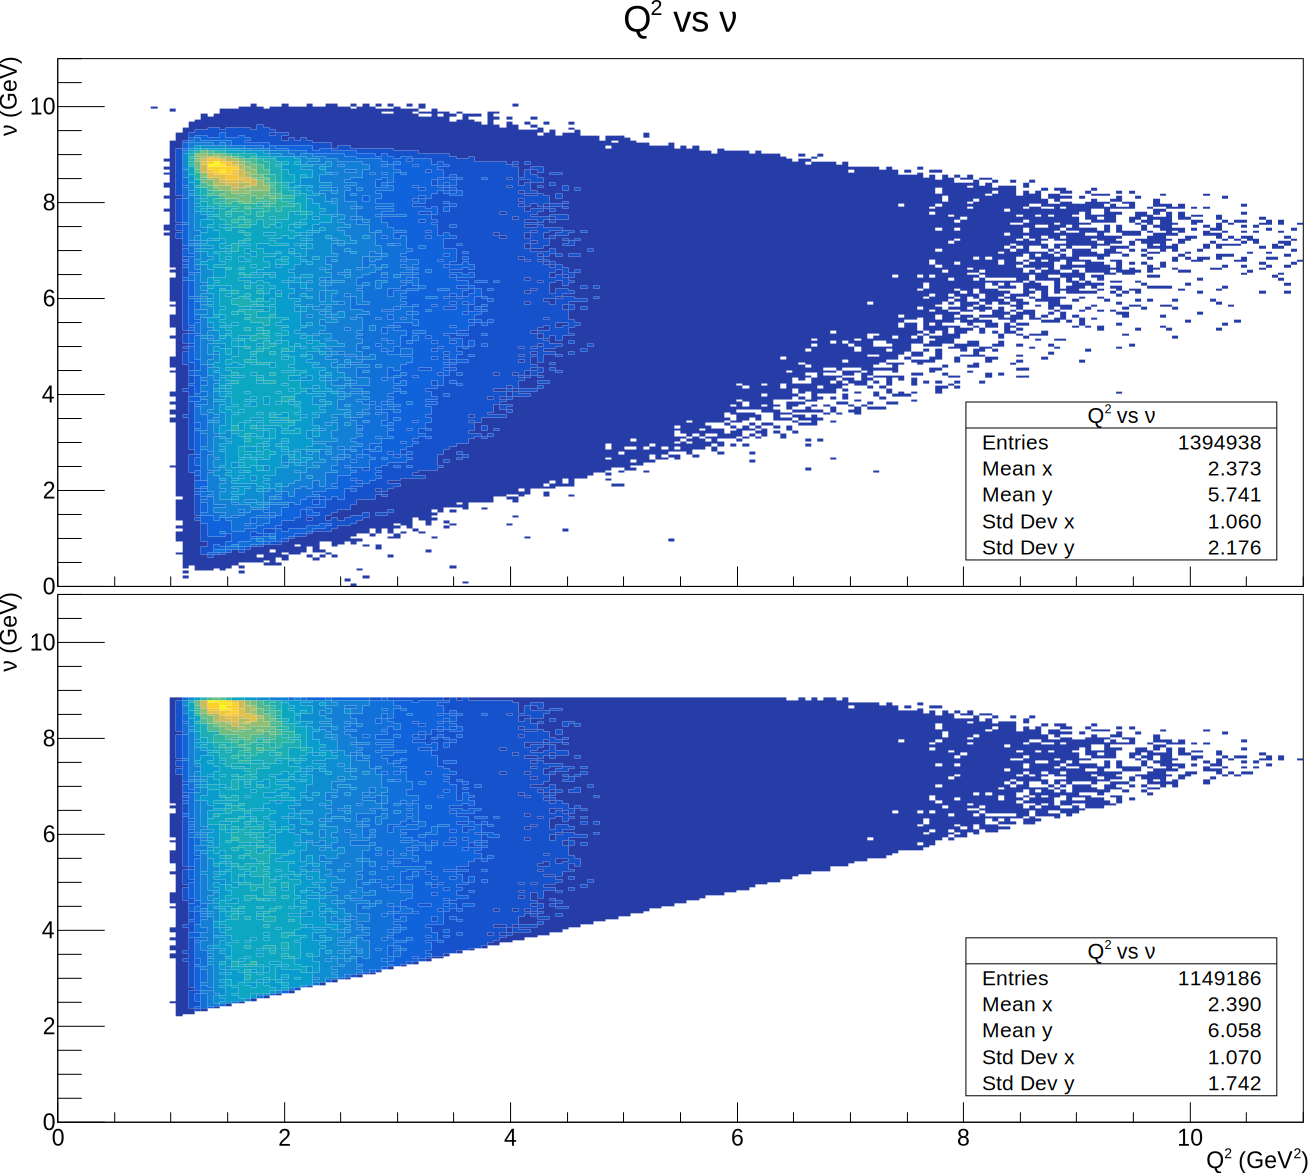
\includegraphics[width=\textwidth]{23q2_vs_nu.pdf}}
        \caption[$Q^2$ vs $\nu$ comparison]{$e^-$ $Q^2$ vs $\nu$ before and after applying the $Q^2 > 1 \text{ GeV}^2$, $W^2 > 4 \text{ GeV}^2$, and $Y_b < 0.85$ cuts, run 12016.
        Source: Own elaboration, using the \hyperlink{github.com/bleaktwig/clas12-rge-analysis}{clas12-rge-analysis} software.}
        \label{fig::q2vsnu}
    \end{figure}

